\setlength{\tabcolsep}{10pt}
In this section, we will focus on additive manufacturing for metal lattice structures using a PBF process. In section \ref{sec:pbf_proc}, we will discuss how 3d printers for PBF process with metal materials, while in section \ref{sec:lattice}, we will delve into lattice structures.
\section{Powder Bed Fusion Processes}\label{sec:pbf_proc}
As we have already discussed in section \ref{sec:AMproc}, powder bed fusion processes can be further divided into laser powder bed fusion also called selective laser sintering (SLS) or electron beam powder bed fusion also called electron beam melting (EBM). Despite the fact that the two technologies are based on two different ideas and some differences in components between 3D printers, the two processes share several common elements and points. Since the thesis concerns lattice structures printed in metal, in this section we will delve into PBF technologies suitable for metallic materials. 
\begin{figure}[H]
    \centering
    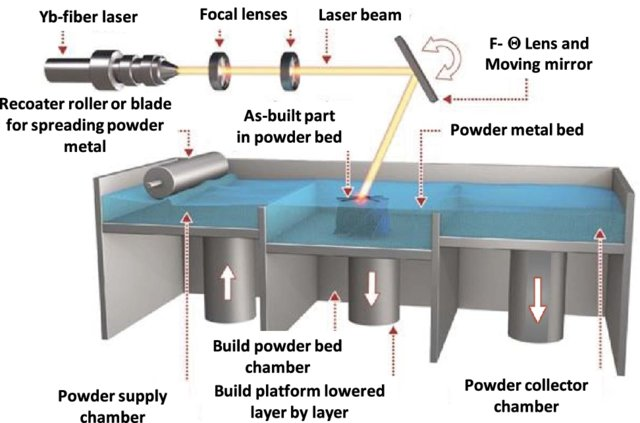
\includegraphics[scale=1.3]{Images/PBF.jpg}
    \caption[PBF in AM.]{Powder bed fusion process in additive manufacturing. Adapted from \cite{ozel_focus_2020}.}
    \label{fig:PBF}
\end{figure}

All PBF 3D printers consist of two basic components: the powder bed, which is a movable container along the z-axis for the metallic powder, and a highly concentrated energy source. 
Firstly, the plate mounting is calibrated and a vacuum is created inside the printer's process chamber or a regular flow of inert gas is introduced to obtain controlled and uniform melting. In the industrial context, directing an inert gas is preferred to maintaining a vacuum throughout the printing process. This is because it's difficult to maintaining a vacuum throughout the printing process and lowering the pressure in the process chamber can lower the boiling point of the metals, leading to the formation of an excessive amount of vapor, which can affect the effectiveness of the laser. Once the vacuum or inert gas flow is established, the roller or blade responsible for distributing the powder performs a rapid powder recoating and an electric resistance located under the powder bed preheats the powder at a temperature of \SI{500}{\degreeCelsius}. This operation help to reduce the gap between the temperature of the chamber and the metal's melting temperature. However, the preheating operation is not always necessary, and in the case of EBM, it is not even required. We will discuss the reason why later. after which the printing can begin. After these preliminary operations, the printing process can begin. A scanning system composed of a laser diode and a galvanometric mirror system selectively melts the metal layer by layer, alternating with the powder distribution tool on the print bed, layer after layer. LASER is an acronym that stands for "Light Amplification by Stimulated Emission of Radiation," and it is a monochromatic beam of photons characterized by low divergence and a focal spot size of \SIrange[range-phrase = --]{30}{80}{\micro\metre}.
\begin{figure}[H]
    \centering
    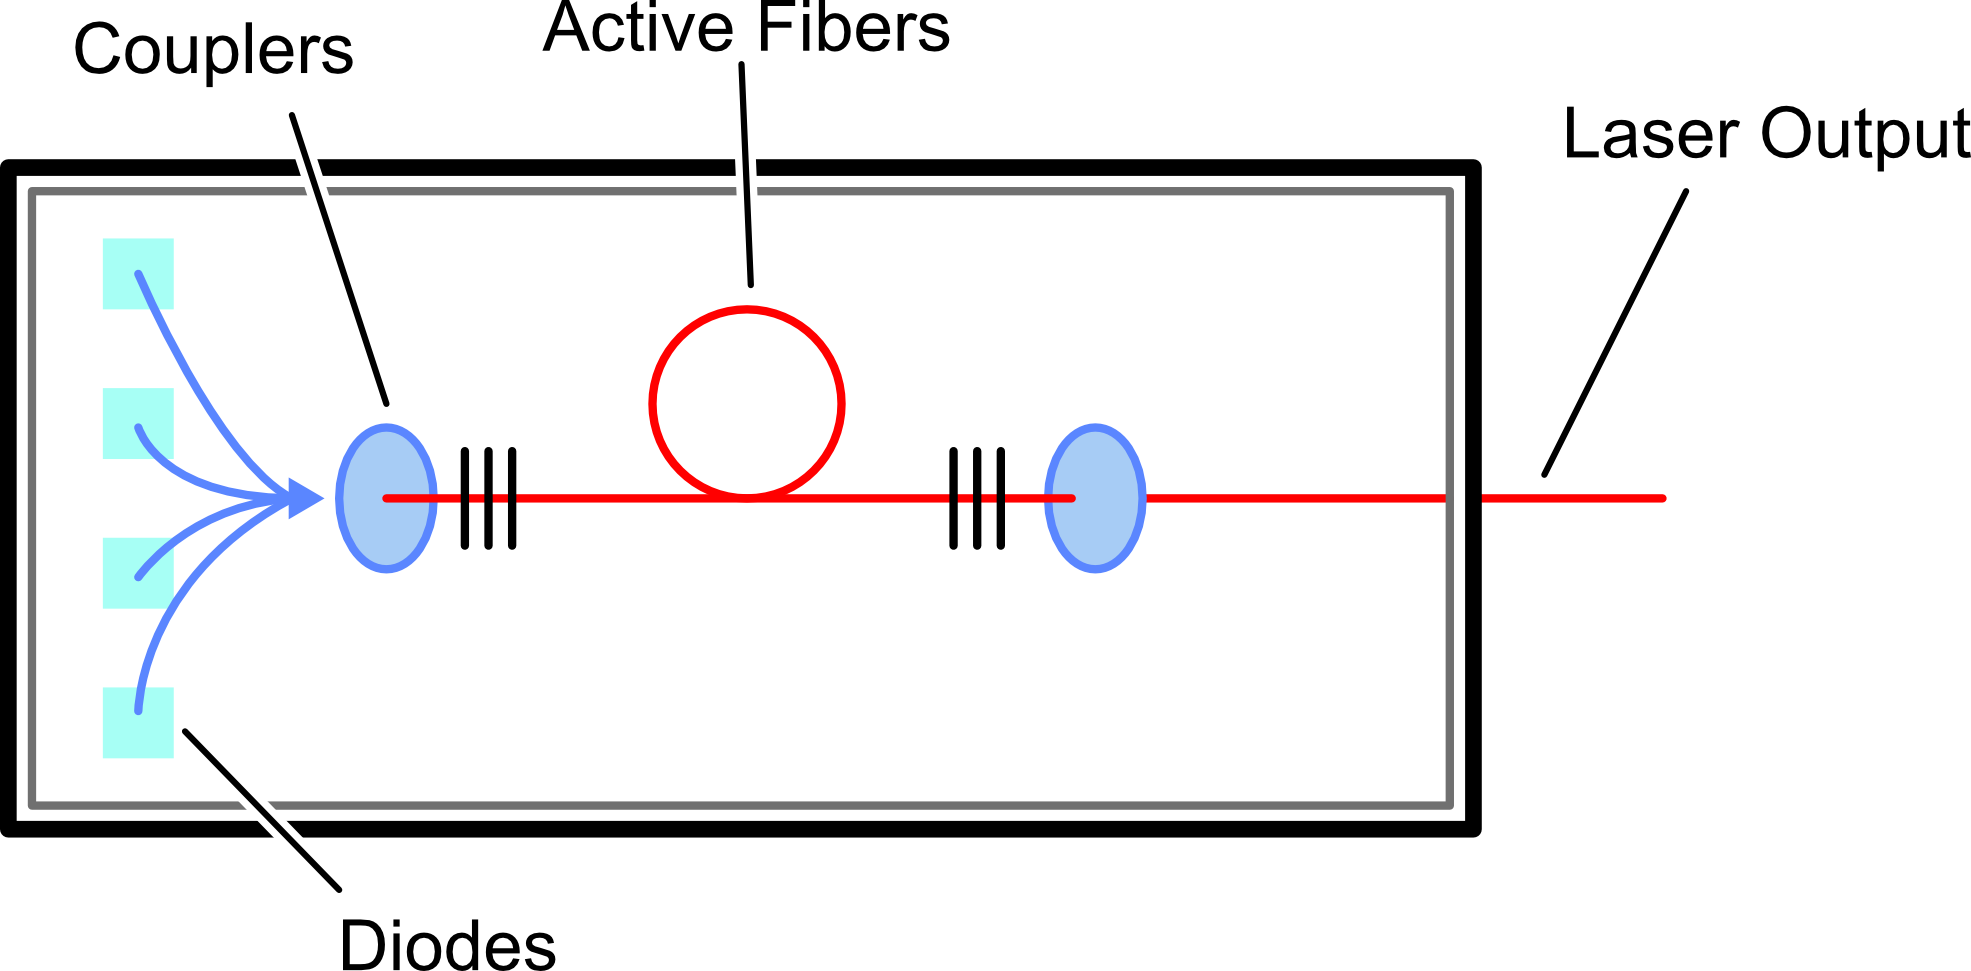
\includegraphics[scale=0.5]{Images/laser2.png}
    \caption[Laser schema.]{Active fiber laser schema.}
    \label{fig:laser}
\end{figure}
Laser equipment has the capability to generate powers in the range of thousands of watts and can focus to beam spot sizes of fractions of a millimeter. These small spot sizes have the potential to create minuscule molten pools that can melt at extremely high travel speeds, reaching up to several meters per second. Nowadays, almost all lasers used in AM rely on active optical fiber sources, fig. \ref{fig:laser}. In this laser technology, optical pump diodes are coupled to an active laser fiber that has a unique reflective coating and Bragg gratings. These components enable the laser light to reflect back-and-forth along the length of the fiber, producing a coherent beam of light at the output of the laser. Additional optical fibers are commonly used to deliver and contain the light energy, providing a robust, flexible, and fully enclosed beam path for beam delivery \cite{milewski_additive_2017}. The energy transferred from the laser to the powder bed depends on the laser power (\SIrange[range-phrase = --]{100}{1000}{\watt}, the light-absorbing capacity of the material, and the scanning speed, which can be controlled by modifying the angular velocity of the galvanometer.

\begin{figure}[H]
    \centering
    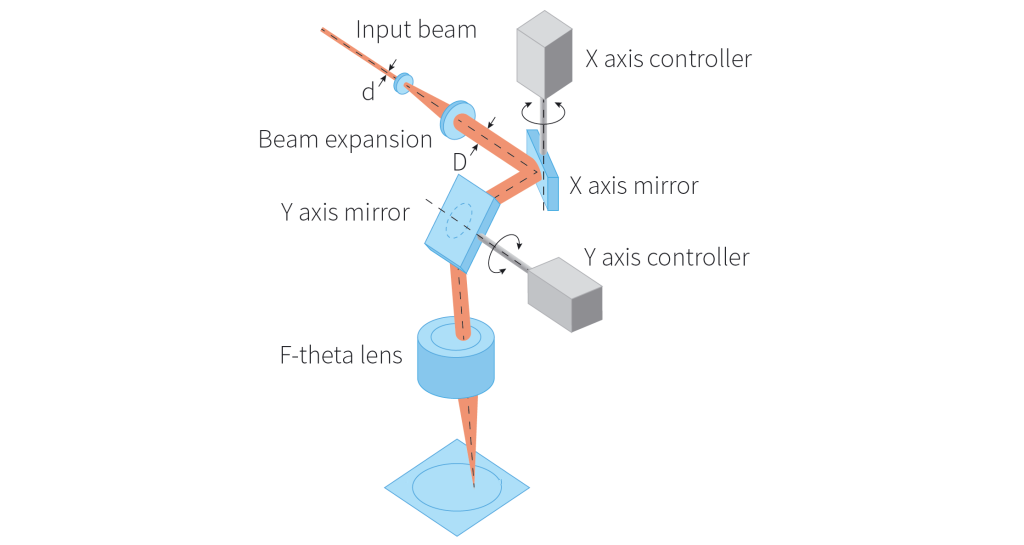
\includegraphics[scale=0.5]{Images/galvanometro.png}
    \caption[Galvanometric system.]{Doul-axis galvanometric system.}
    \label{fig:galvano}
\end{figure}
The galvanometric system, fig. \ref{fig:galvano}, system consists primarily of two mirrors rotating along their axis, enabling the laser beam to be directed, and a series of f-theta lenses that facilitate rapid laser movement and precise focusing of laser beam. After completing the printing process, it is necessary to allow the object to cool down. Although supports are not always necessary in PBF processes as the powder gives support to the object itself, they may need to be inserted to ensure uniform heat transmission during both the printing and cooling processes. Once the object has cooled down, any excess powder can be removed. The excess powder can be recycled and reused after undergoing some preliminary processing and conformity controls. Finally, if required, post-processing operations can be carried out, such as removing any supports, surface finishing, and annealing. This is especially important if the cooling process inside the chamber has created an undesired microstructure in the final cooling part.\\
In EBM printers, the process is fundamentally the same as in laser printers, with metal powder selectively fused from a tray. However, there are several significant differences. Firstly, the energy source is not a laser (i.e., a beam of photons) but rather an electron beam. Secondly, the preheating stage is not accomplished through the use of an electric resistor, but instead through the use of the electron beam itself. But how does an electron beam function? To produce an electron beam, an electric current is passed through a tungsten filament. The resulting electron beam is then directed through a Wehnelt cylinder, which, when negatively or positively charged, respectively blocks or allows the passage of electrons.

\begin{figure}[H]
    \centering
    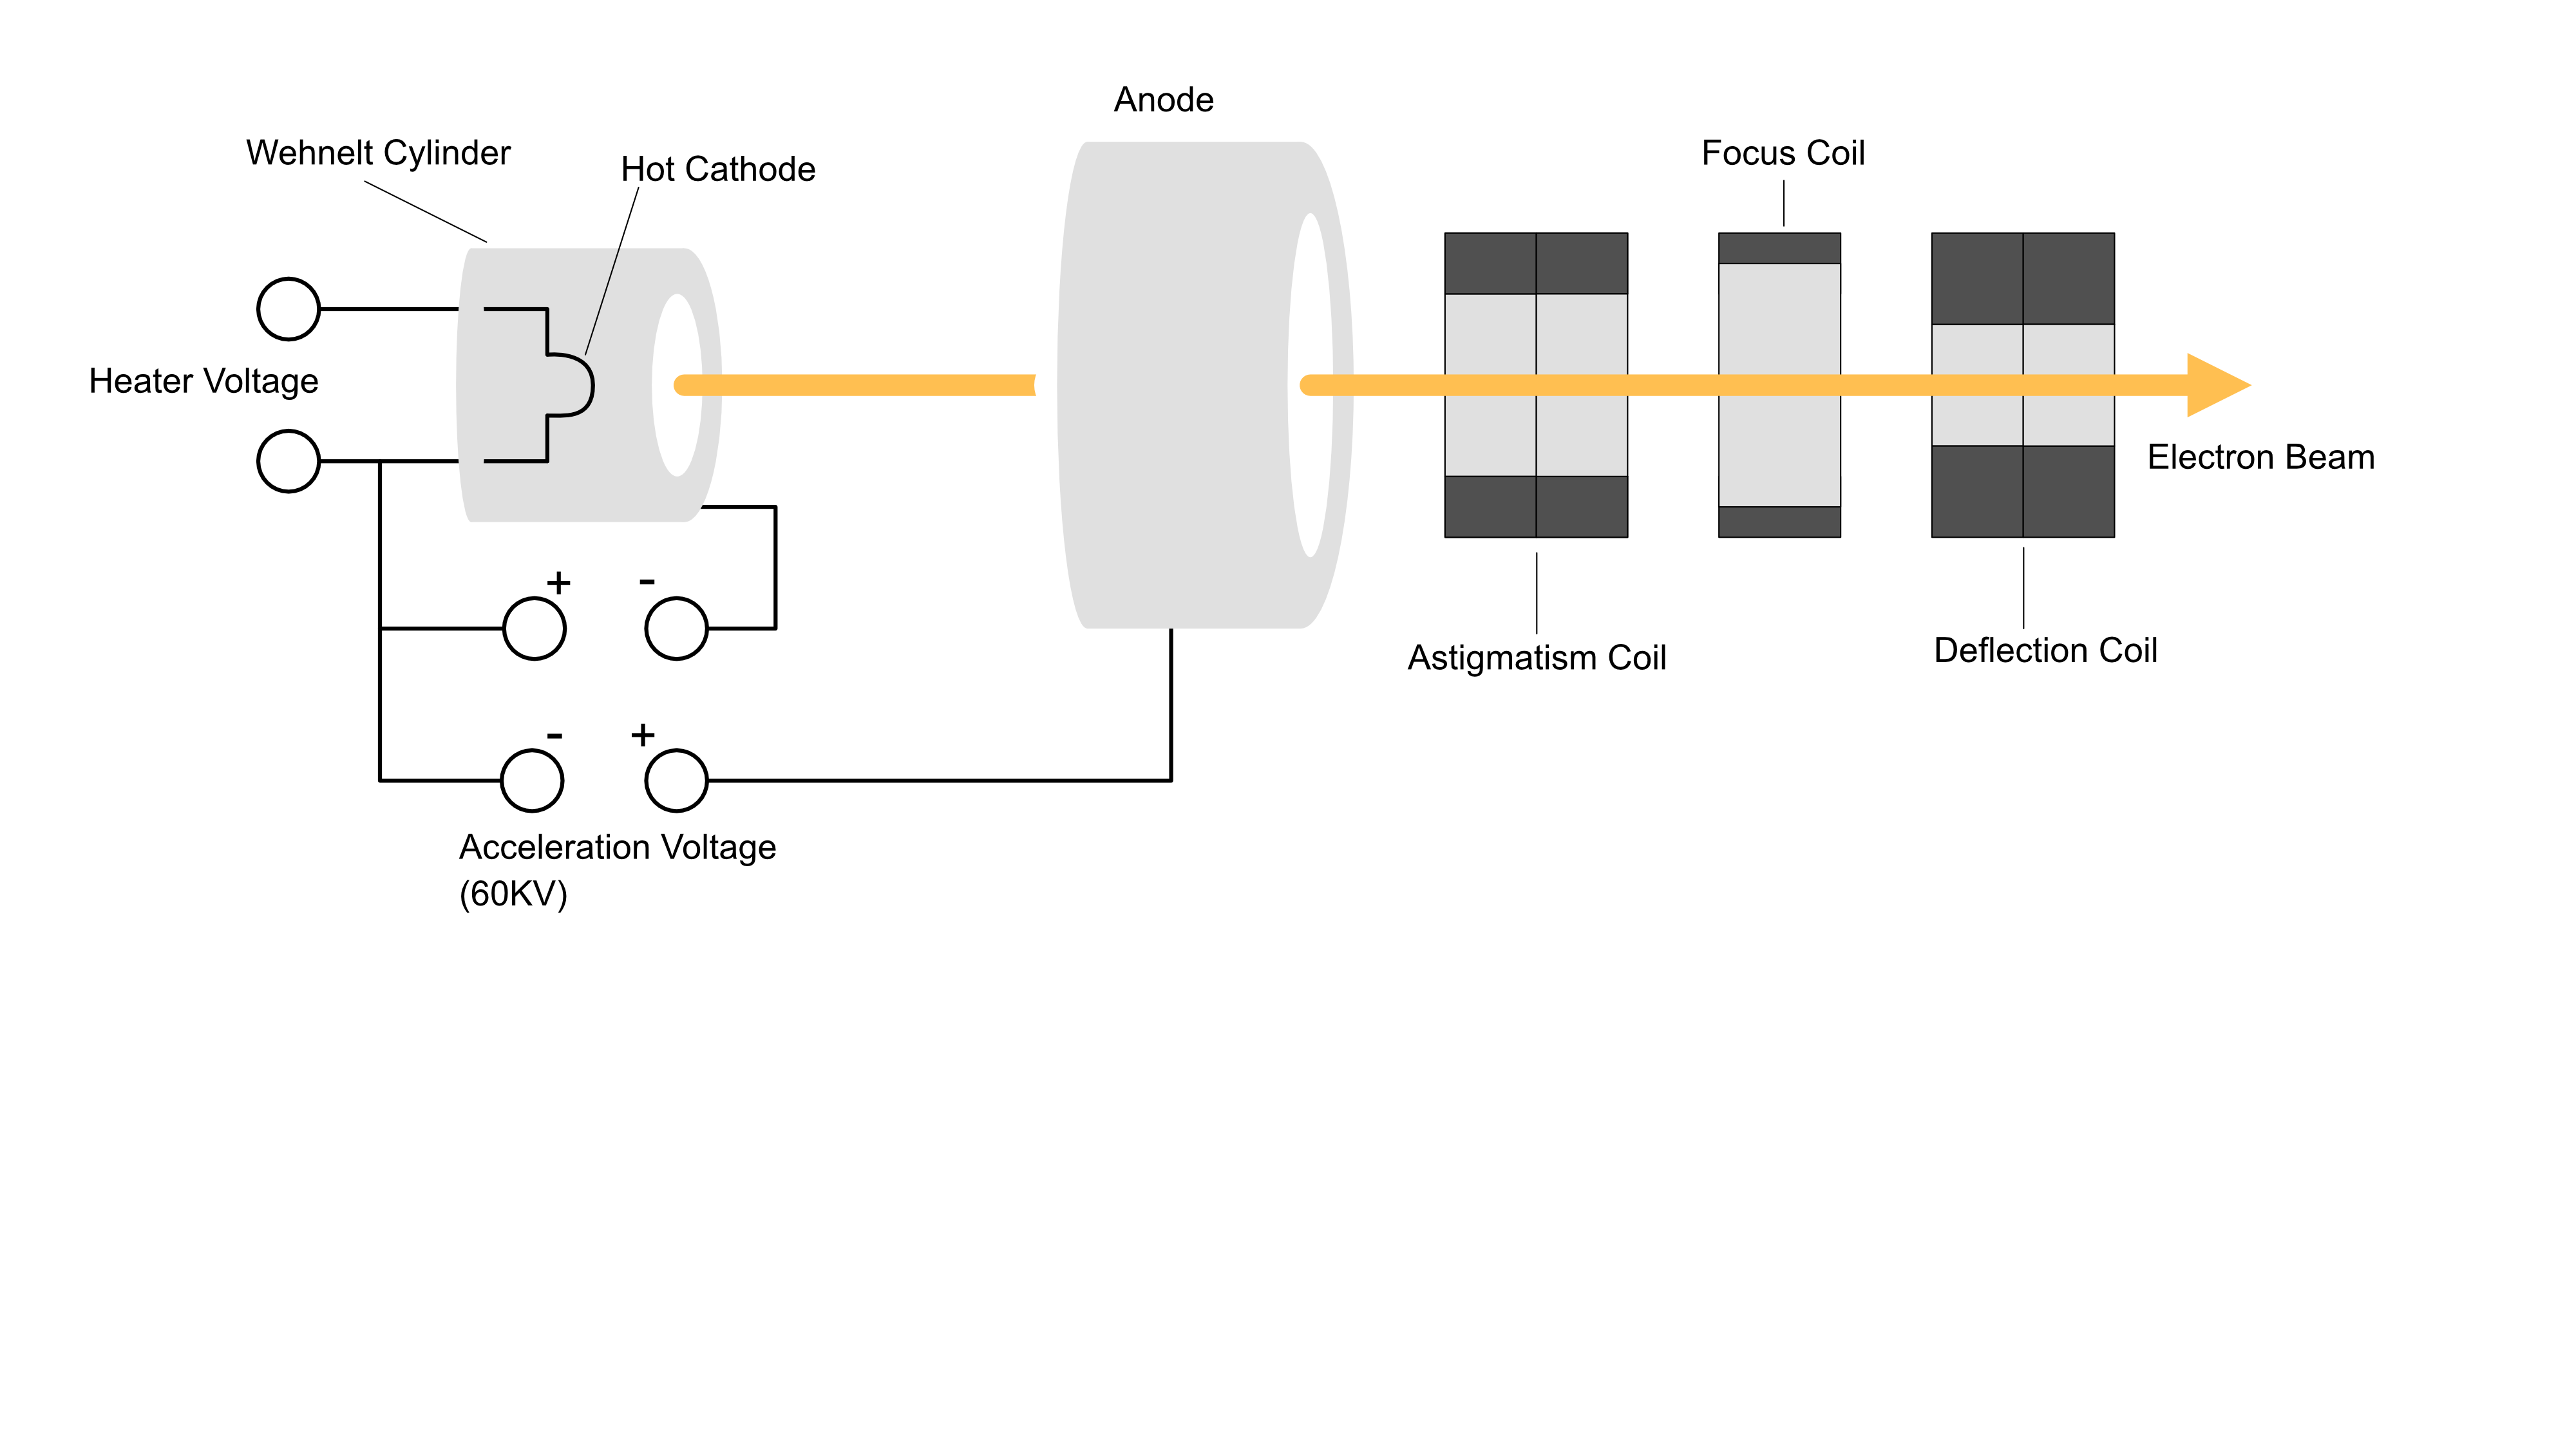
\includegraphics[scale=0.5]{Images/EBM.png}
    \caption[Electron gun schema.]{Electron gun schema.}
    \label{fig:electrongun}
\end{figure}

A diagram of the electron gun beam's structure can be seen in fig. \ref{fig:electrongun}. Finally, the electron beam passes through an anode charged with a voltage of up to \SI{60}{\kilo\Volt}, which accelerates the electrons and allows the beam to be directed into the column through magnetic lenses. Unlike SLS printers that use optical lenses, the lenses in EBM printers are magnetic and use a magnetic field to alter the path of the electron beam. As the beam passes through these lenses, the astigmatic lenses adjust the shape of the electron beam spot, the focus coil changes the spot size, and the deflection coil moves the beam along the x and y axes. Like SLS printers, the EBM printer requires a vacuum inside the printing chamber, and a minute amount of helium must be continuously injected into the chamber to prevent the accumulation of electric charges due to any residual electrons on the powder bed. To put the minuscule amount of helium required into perspective, consider that the starting pressure is \SI{0,0005}{\milli\bar}, and the pressure with helium flow is bout \SI{0,002}{\milli\bar}.


%%%%%%
%%%%%%
\section{Metal Powders for AM} \label{sec:metalpowders}
As we have seen in the section \ref{sec:pbf_proc}, PBF processes require metal powder for the process. Various metallic materials can be transformed into powders suitable for use in additive manufacturing processes, and can be applied in different sectors according to their mechanical properties. The table \ref{table:materialAMmetal} presents some examples of metallic materials that can be used for this purpose. 

\begin{table}[H]
\centering 
    \begin{tabular}{|l l l|}
    \hline
%    \rowcolor{bluepoli!40}
     \textbf{Material} & \textbf{Examples} & \textbf{Applications}\\
    \hline \hline
    \textbf{Stainless steel} & 316L, 174-PH, MS1, M300 & Food, biomedical, consumer \T\B\\
    \hline
    \textbf{Ni-alloys} & In625, In718, In939 & Energy, motorsport\T\B\\
    \hline
    
    \textbf{Al-alloys} & AlSi12, AlSi10Mg & Lightweight, aerospace, aviation\T\B\\
    \hline

    \textbf{CoCr-alloys} & CoCrMo & Dental, biomedical\T\B\\
    \hline

    \textbf{Ti-alloys} & Ti6Al4V, CP Ti & Biomedical, lightweight, aerospace\T\B\\
    \hline

    \textbf{Tool steel} & Maraging 18Ni300 & Tooling, aerospace, automotive\T\B\\
    \hline

    \textbf{Cu-alloys} & Bronze & Energy, heat exchanger\T\B\\
    \hline

    \textbf{Precious} & Au, Pt, Ag & Jewellery, design\T\B\\
    \hline
    
    \end{tabular}
    \\[10pt]
    \caption{Material availability for metal AM.}
    \label{table:materialAMmetal}
\end{table}




In the vast majority of cases, these powders are produced using atomization processes that exploit various physical methods to generate micro-particles characterized by a spherical shape and of which chemical purity depends on the method used. The inefficiency and cost of atomization processes used for manufacturing metal powders is the reason why, in the case of specific high-quality powders, the powder price can be up to 10 times the price of raw metal. It has been demonstrated that powders made of irregular microparticles with low chemical purity can lead to structural defects in the final parts, resulting in lower performance \cite{deng_origin_2020}. Therefore, over the years, increasingly complex and expensive processes have been developed to obtain higher-quality powders. In figure \ref{fig:atom} there are various atomization processes schematically depicted.
\begin{figure}[H]
    \centering
    \subfloat[Water atomization process.\label{fig:wateratom}]{
        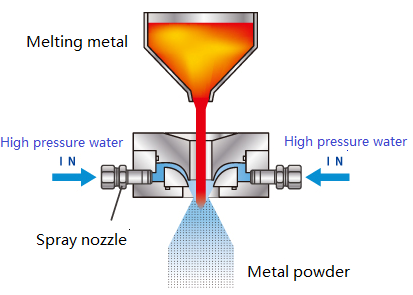
\includegraphics[scale=0.6]{Images/wateratom.png}
    }
    \qquad
    \subfloat[Gas atomization process.\label{fig:gasatom}]{
        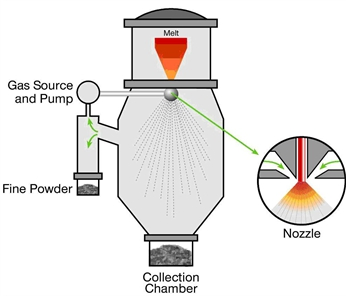
\includegraphics[scale=0.6]{Images/gasatom.png}
    }
    \qquad
     \subfloat[Plasma atomization process.\label{fig:plasmaatom}]{
        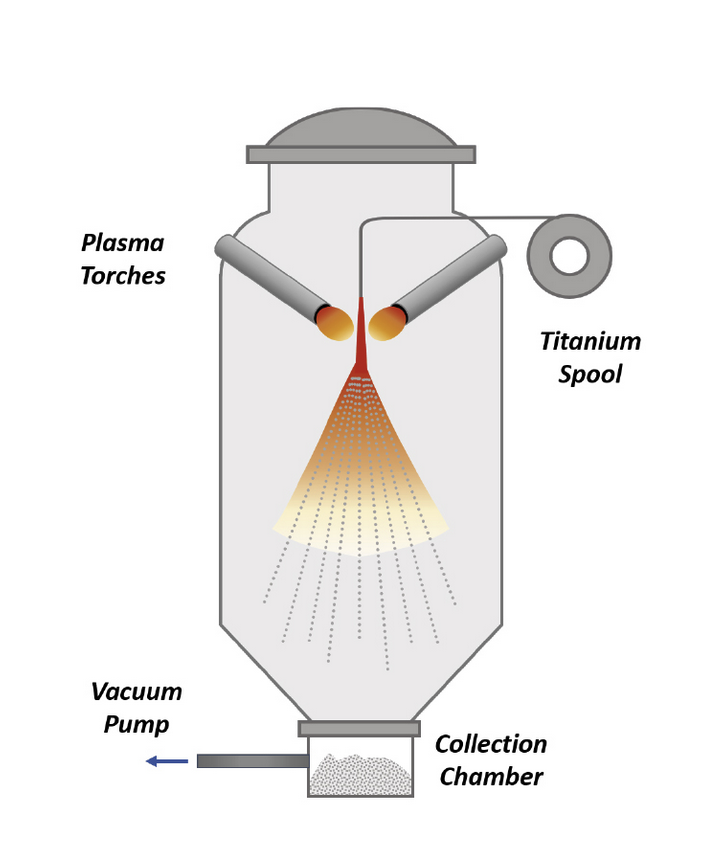
\includegraphics[scale=0.4]{Images/plasma.png}
    }
    \qquad
    \subfloat[Rotating electrode process.\label{fig:repatom}]{
        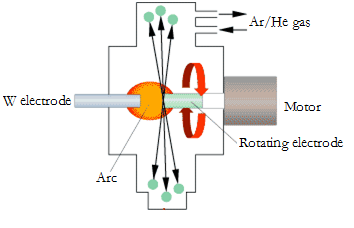
\includegraphics[scale=0.7]{Images/repatom.png}
    }
    
    \caption[Atomization processes]{Different atomization processes. Pictures from \cite{material_technology_innovations_co_rotating_nodate, material_technology_innovations_co_water_nodate, material_technology_innovations_co_gas_nodate, inovar_communications_ltd_metal_2020}.}
    \label{fig:atom}
\end{figure}
The process of \emph{water atomization}, fig. \ref{fig:wateratom}, of metals involves the production of small droplets of molten metal by exposing a stream of the molten metal to a high-pressure jet of water. The water atomization process is typically carried out in a chamber where the molten metal is injected into a nozzle that directs the stream of liquid metal towards a high-pressure jet of water. As the molten metal comes into contact with the water, it rapidly cools and solidifies, forming small droplets that are collected at the bottom of the chamber. The size and shape of the metal droplets produced during the water atomization process can be controlled by adjusting various parameters such as the temperature of the molten metal, the pressure of the water jet, and the distance between the nozzle and the water jet. By controlling these parameters, it is possible to produce metal powders with a range of particle sizes between \SIrange[range-phrase = --]{1}{500}{\micro\metre}. The output-to-input ratio for this process is approximately 95\%, which means that from \SI{1}{\kilo\gram} of raw metal, it is possible to obtain up to \SI{950}{\gram} of powder. Compared to other powder production methods, the water atomization process offers several advantages including high production rates, the wide range of particle sizes obtainable, high production rates, and the fact that metal ingots can be used as process input, which shortens the supply chain of this production process. On the other hand, the major disadvantages are the low chemical purity, irregular shape as can be seen in fig. \ref{fig:waterpow}, and the need for extensive post-processing to obtain a decent-quality product. Moreover, it cannot be used with reactive materials such as titanium and aluminum.

\emph{Gas atomization}, fig. \ref{fig:gasatom}, can be performed using a variety of gases, depending on the specific application and metal being processed. The most commonly used gases for gas atomization are inert gases such as nitrogen, argon, and helium, even if the latter is barely used in industrial applications due to its high cost. Inert gases are preferred because they do not react with the molten metal and do not introduce impurities into the metal powders. Metal ingots are molten and the flow is rapidly solidifying through exposure to a high-pressure stream of gas. Main advantages of this process are the high production rate, the wide range of obtainable particles, its applicability to reactive materials, and its ability to ensure good chemical purity. The main drawbacks, on the other hand, are mostly related to the porosity of the resulting powder and the formation of small satellite particles. Additionally, the cost of the process is higher if compared to water atomization.

The process of \emph{plasma atomization}, fig. \ref{fig:wateratom}, involves the usage of high-temperature plasma torches to melt metal wire. The high-energy plasma arc is created by passing an electric current through a non-consumable tungsten electrode and an inhert gas jet to direct the welding arc into a focused area. As the molten metal droplets are expelled from the plasma jet, they rapidly solidify, sometimes also thanks to the water-cooled chamebr, and break up into small, spherical powders, which are then collected in a container. The plasma atomization process offers several advantages over other powder production methods, including the ability to produce powders from reactive metals and the ability to produce extremily spherical shape. Plasma atomization can also produce powders with very high purity levels, as the high temperature of the plasma jet helps to eliminate impurities in the molten metal. However, plasma atomization is more expensive than other powder production methods due to the need for specialized equipment and the high energy consumption required to generate the plasma arc. The process can also be challenging to control, as variations in process parameters can affect the size, shape, and purity of the resulting metal powders. Lastly, powders produced using this method has a low size range of about \SIrange[range-phrase = --]{1}{200}{\micro\metre}. 

In \emph{rotating electrode process}, a consumable metal electrode is rotated at high speeds while it is melted by an electric arc. As the molten metal is exposed to the high-velocity inert gas stream, it rapidly solidifies and breaks up into small droplets, which are then collected at the bottom of the atomization chamber. Due to its high cost, this production method is typically used when it is necessary to obtain a metal powder with a perfectly spherical shape and without any impurities. If we take a look at fig. \ref{fig:reppow}, we can easily grasp the potential of this technology in obtaining perfect spherical micro-particles.
\begin{figure}[H]
    \centering
    \subfloat[\label{fig:waterpow}]{
        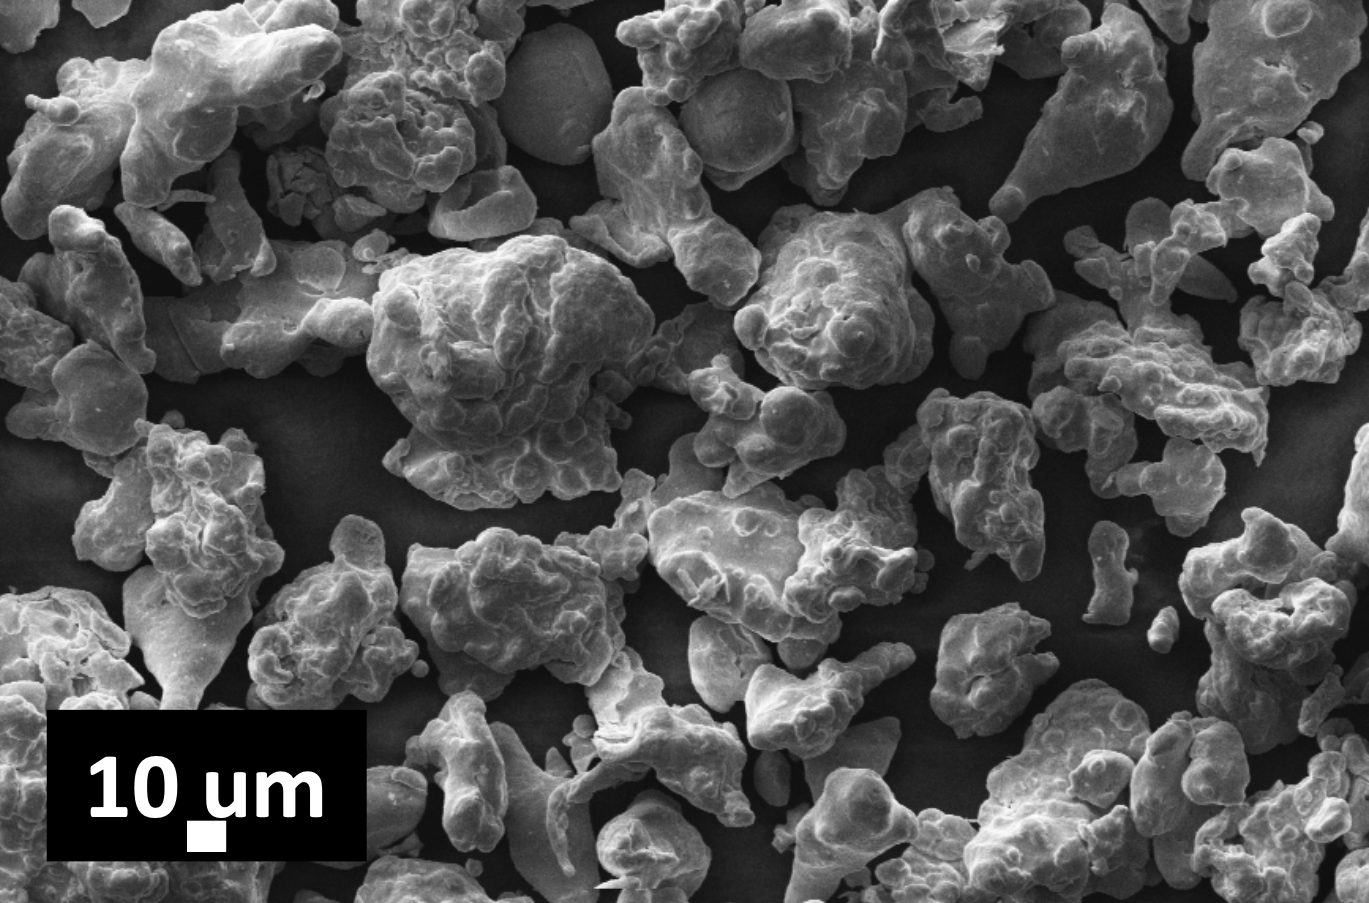
\includegraphics[scale=0.22]{Images/waterpow.png}
    }
    \qquad
    \subfloat[\label{fig:gaspow}]{
        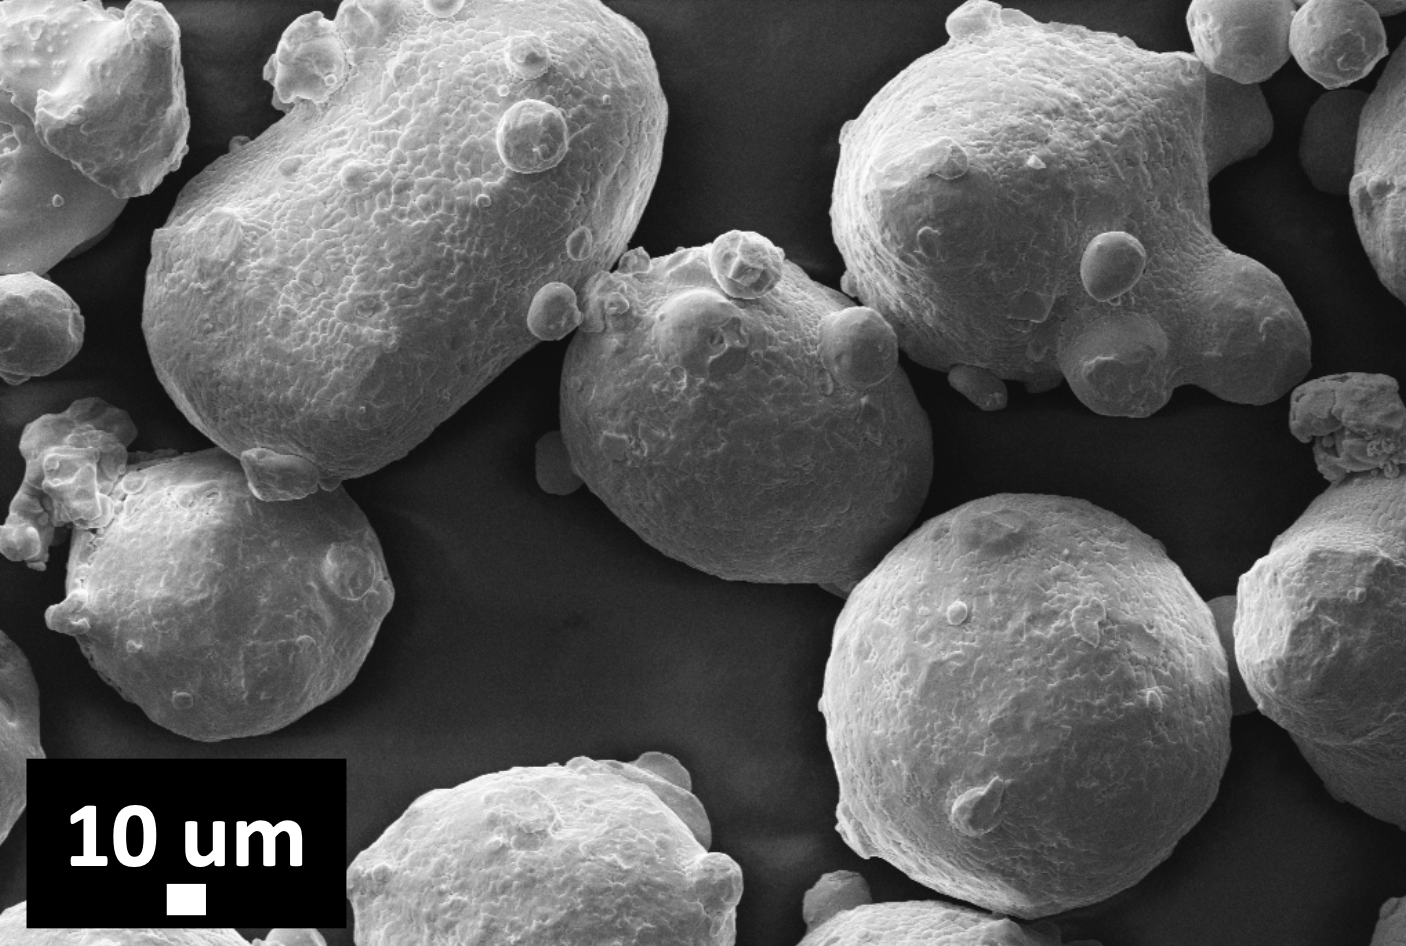
\includegraphics[scale=0.21]{Images/gaspowd.png}
    }
    \qquad
     \subfloat[\label{fig:plasmapow}]{
        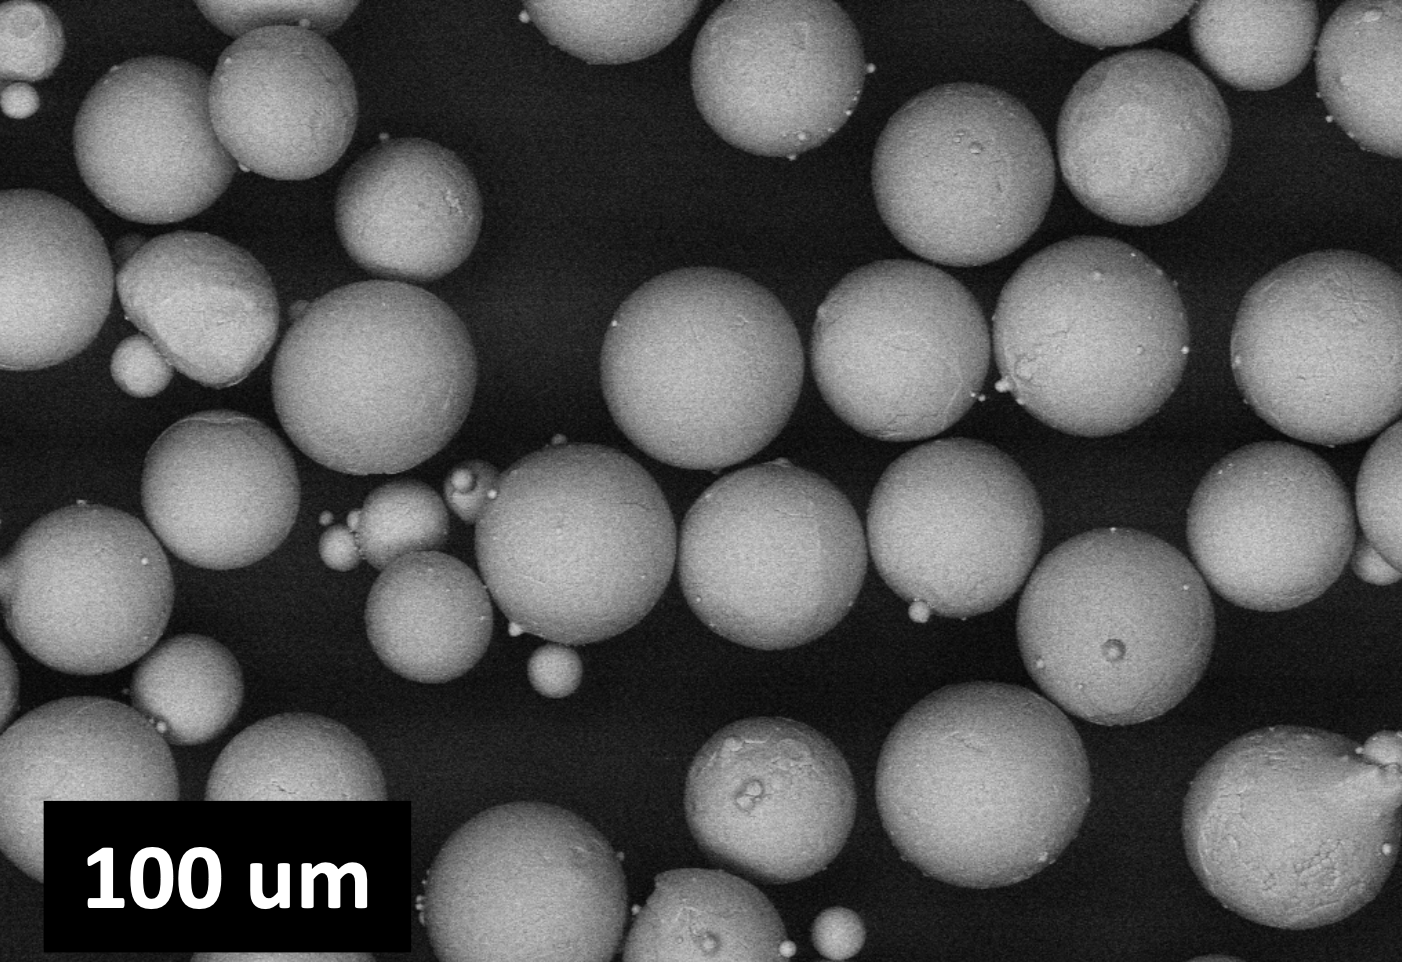
\includegraphics[scale=0.22]{Images/plasmapowder.png}
    }
    \qquad
    \subfloat[\label{fig:reppow}]{
        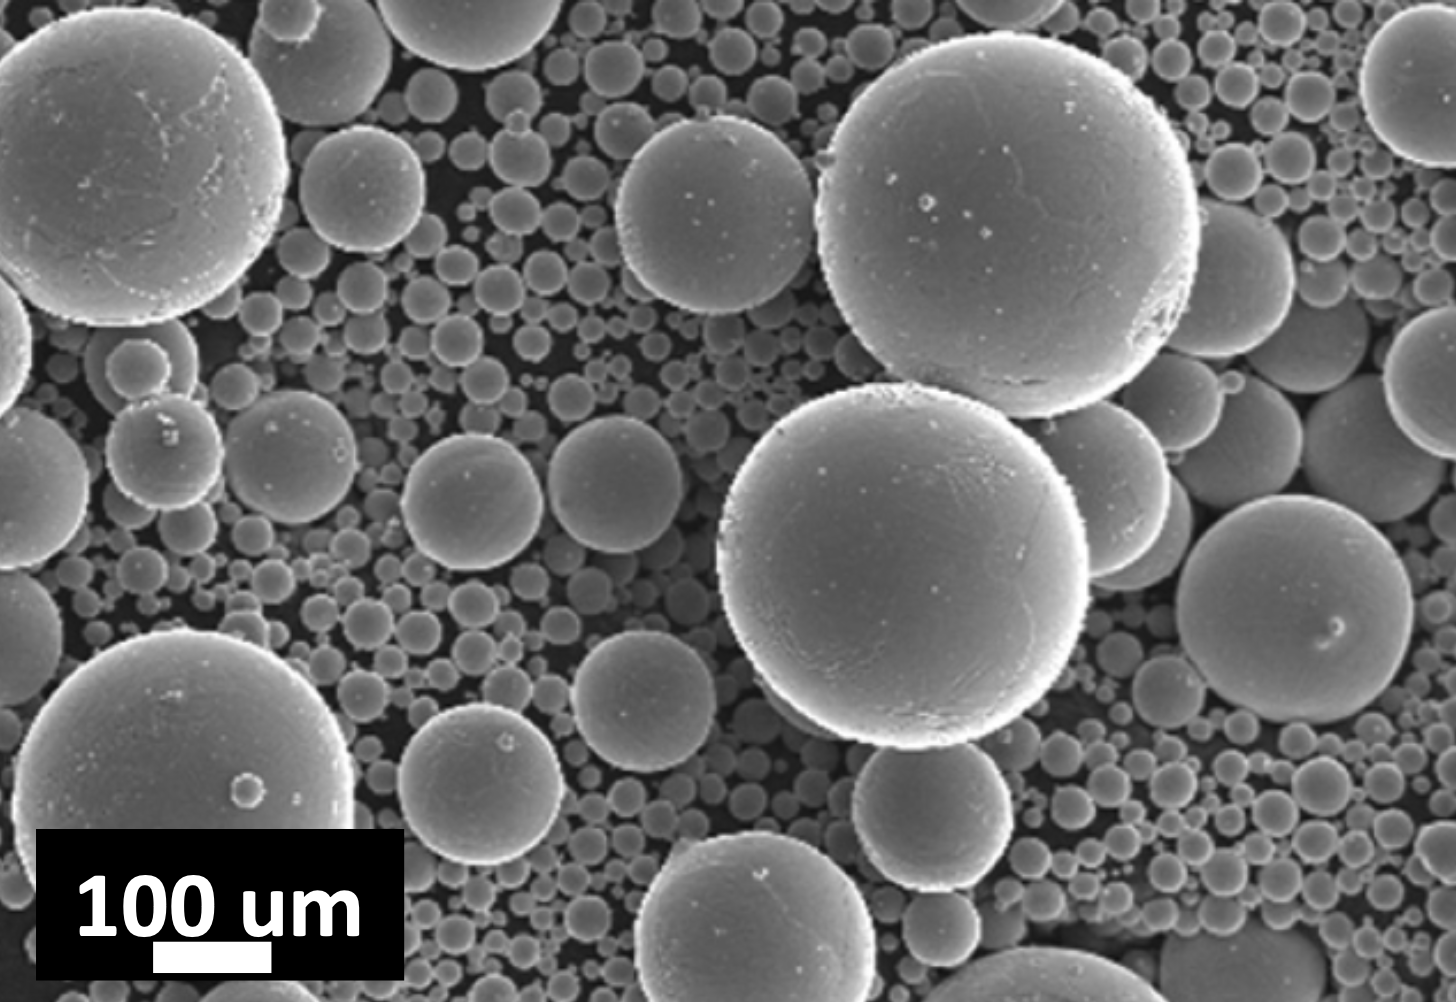
\includegraphics[scale=0.21]{Images/erppowder.png}
    }
    
    \caption[Powders from atomization processes]{Micro-particles obtained by water atomization (a), gas atomization (b), plasma atomization (c) and rotating electode process (d).}
    \label{fig:powders}
\end{figure}
%%%%%%
%%%%%%
\section{Lattice Structure and Cellular Material} \label{sec:lattice}
According to ISO/ASTM 52900 \cite{international_standard_organization_isoastm_2015}, lattice structure are "three dimensional geometric arrangement composed of connective links between vertices (points) creating a functional structure". So, lattice structures are three-dimensional structures made up of different connected single elements called "cells" that can have different shapes, designed to meet the needs of the final object. These objects are distinguished by empty spaces within the structure. These structures can only be obtained thanks to layer-wise additive manufacturing technologies, since they allow us to design and to manufacture objects with complex designs and intricated parts. In recent years, the biomimicry technique has also spread to additive manufacturing, and lattice structures are the natural manifestation of this technique. Biomimicry is a set of design techniques that allow us to take inspiration from nature to find solutions to engineering problems or to design functional components that can be used in engineering applications \cite{pathak_biomimicry_2019, du_plessis_beautiful_2019}. Nature, over the past 3.8 billions years, has been able to find the most efficient way to develop functional solutions to evolutionary problems characterized by immovable constraints, whether they are determined by the organism itself or by external factors. For example, think of the wings of dragonflies in fig. \ref{fig:dragonfly}, a lightweight, completely transparent structure that allows flight, allowing them to fly unnoticed by predators. 
\begin{figure}[H]
    \centering
    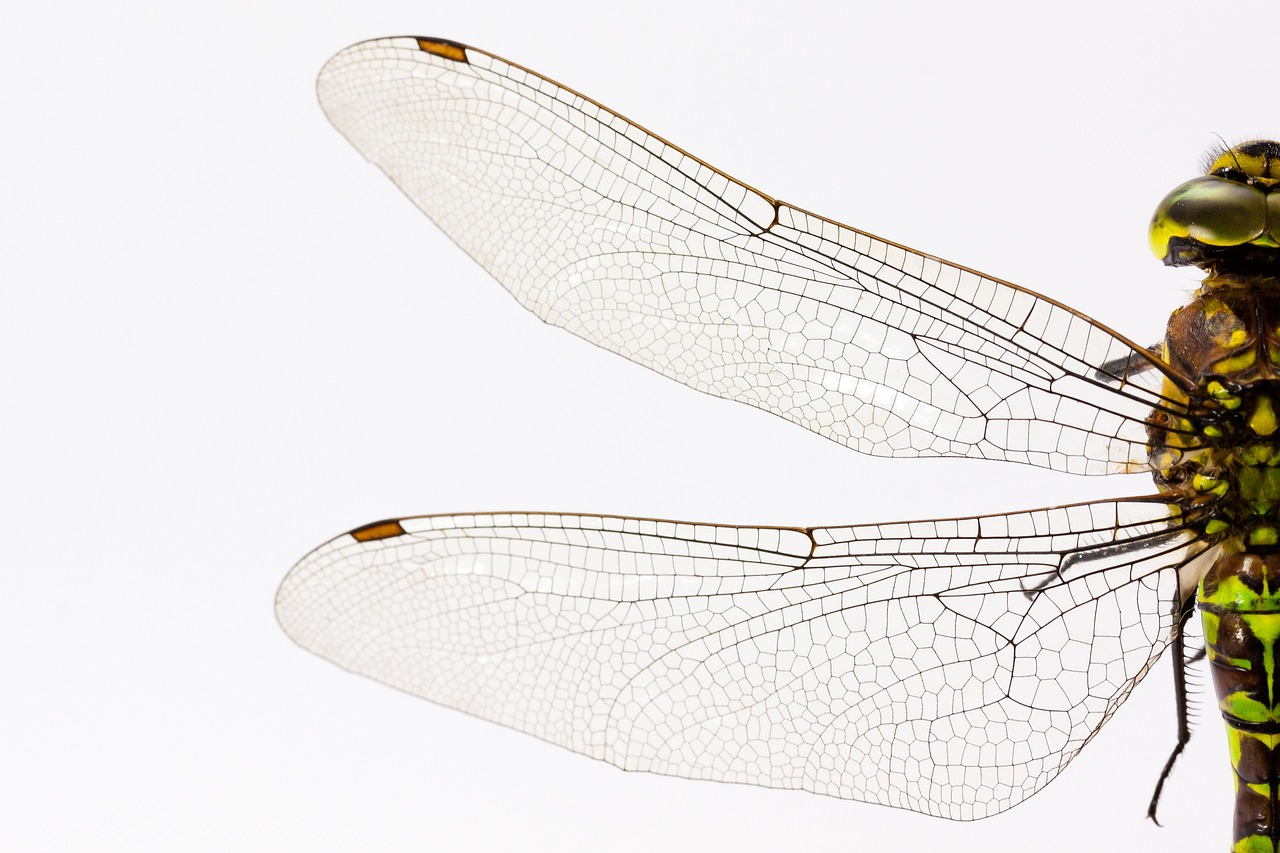
\includegraphics[width=0.45\textwidth]{Images/dragonfly-gf80b992d6_1280.jpg}
    \caption[Dragonfly wings.]{Dragonfly wings are a functional structure constrained by weight.}
    \label{fig:dragonfly}
\end{figure}
Moreover, during the evolutionary process of species, nature has been able to create nano, micro, and macro-structures that provide unique structural properties, adapting shape to function and using only what is truly necessary to achieve the evolutionary goal. Indeed, one of life's principles explained in \citeauthor{baumeister_biomimicry_2011} states \textit{"Life integrates and optimizes these strategies to create conditions conducive to life"}. Therefore, it not only concerns the possibility of creating new multi~-~functional structures with completely new characteristics, but also of doing so by optimizing materials and reducing waste. People have always been fascinated by cellular materials, which is evident from the fact that the first reference to the idea that structure could influence the functional characteristics and behavior of a material was made by Robert Hooke in 1665 \cite{l_gibson_cellular_2010}. Only in recent years, thanks to the computational power of new CAD softwares, it has been possible to experiment with the mechanical characteristics of 3D printed lattice structures. Cellular materials are used mainly for their mechanical characteristics.

\begin{figure}[H]
    \centering
    \subfloat[\label{fig:beehive}]{
        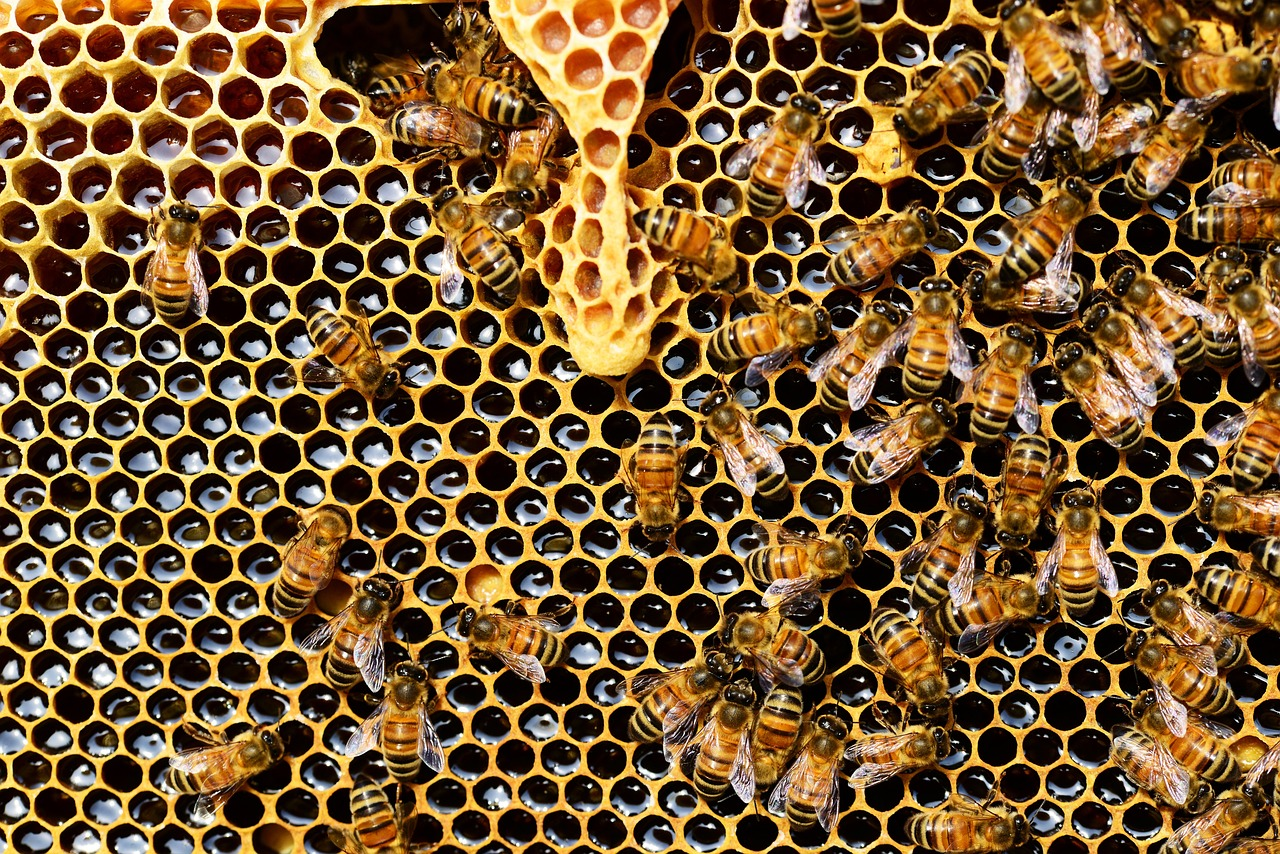
\includegraphics[scale=0.15]{Images/honey-bees-337695_1280.jpg}
    }
    \quad
    \subfloat[\label{fig:beelattice}]{
        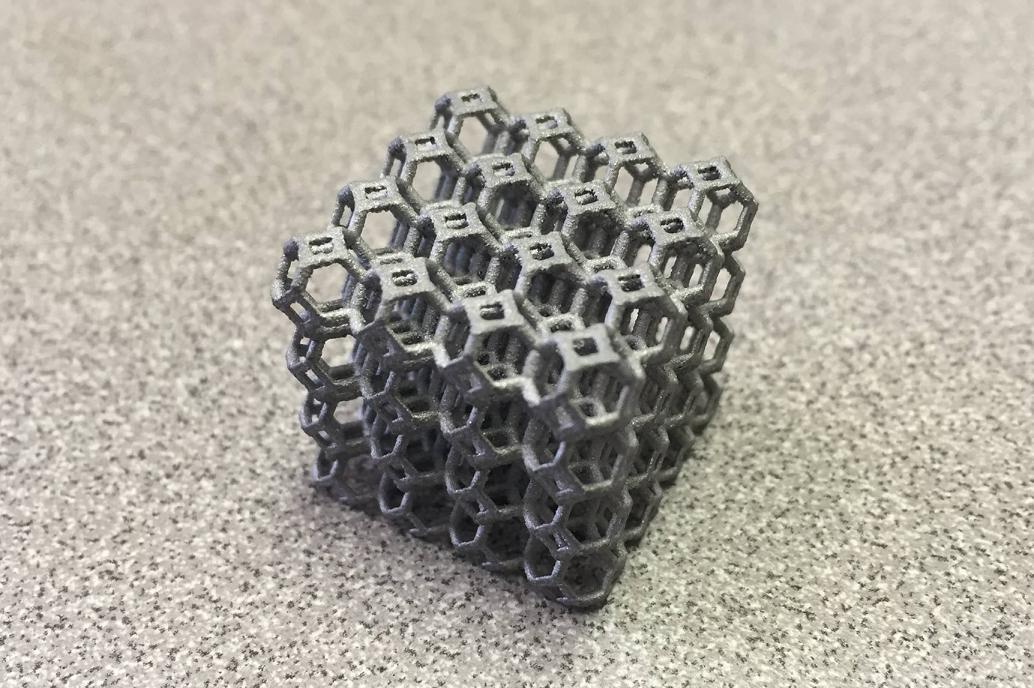
\includegraphics[scale=0.186]{Images/lattice1b.jpg}
    }
    \caption[Bio-inspiration design.]{An example of bio-inspiration design, on the left a beehive and on the right a lattice structure.}
    \label{fig:bioinsp}
\end{figure}

Just think that the aluminum cube in fig. \ref{fig:beelattice} was printed using only \SI{3.9}{g} of material and is able to support a weight of \SI{408}{Kg}, which means it can withstand a stress 100,000 times its weight \cite{noauthor_3d_2014}. If we want to provide a more rigorous framework for classifying the applications of lattice structures in engineering, we can refer to the one proposed by \citeauthor{mcnulty_framework_2017}. According to this framework, cellular structures in nature exist primarily for three reasons:
\begin{itemize}
    \item \textbf{3D space-filling structures}, maybe this is the reason that most closely links the use of cellular structures in nature with AM, namely the need to confer strength to the structure while limiting its weight. Examples of this are the beehive, whose structure provides it with High specific stiffness under self-weight, or toucan's beak in fig. \ref{fig:tucanostruct}, which is characterized by an high bending stiffness;
    \item \textbf{Surface structures}, are structure which enable surfaces to gain specific functional characteristics. For example, veining on the underside of the Amazon water lily leaf in fig. \ref{fig:leafstruct} allows the leaf to gain excellent mechanical resistance, while pomelo skin in fig. \ref{fig:pomelostruct}, with its open-cell structure, enables the fruit to resist impacts;
    \item \textbf{Cylindrical structures}: there are also examples of the use of cellular materials to confer particular characteristics to cylindrical structures (often hollow structure) that would otherwise be too fragile. For example in fig. \ref{fig:hedgehogstruct} there is a hedgehog quill and the particular structure confers ovalization and buckling resistance to the structure and in fig. \ref{fig:bananostruct} there is the section of the petiole of a banana, which is characterized by an high bending stiffness but also a torsional flexibility.
\end{itemize}
\begin{figure}[H]
    \centering
    \subfloat[Toucan beak section.\label{fig:tucanostruct}]{
        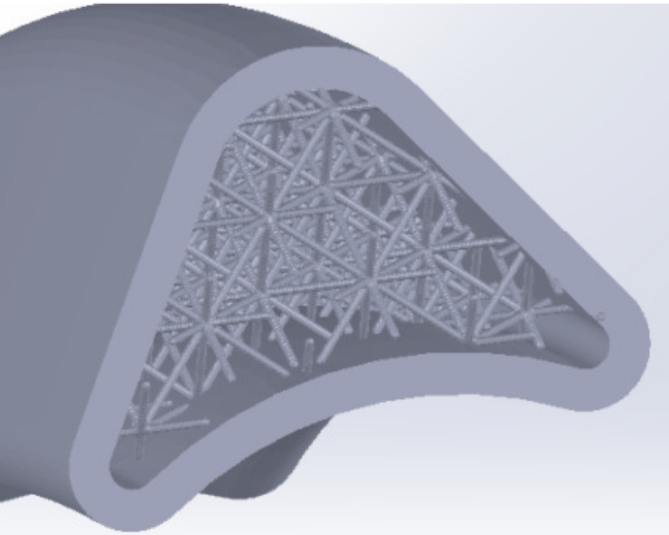
\includegraphics[scale=0.4]{Images/tucano.png}
    }
    \qquad
    \subfloat[Amazon Waterlily leaf underside.\label{fig:leafstruct}]{
        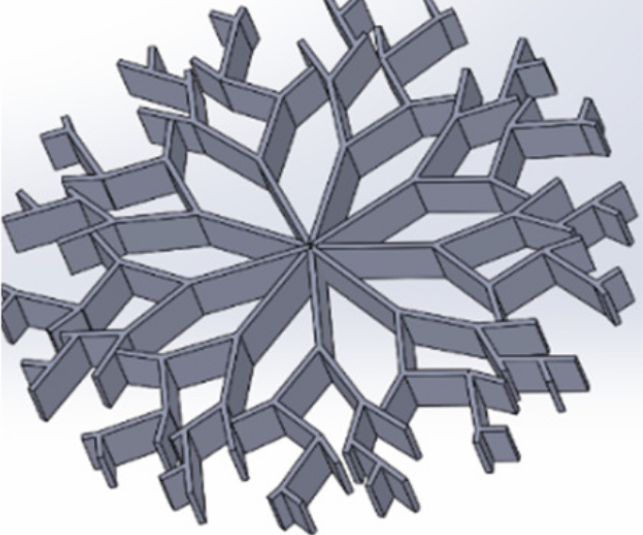
\includegraphics[scale=0.4]{Images/leaf.png}
    }
    \qquad
     \subfloat[Pomelo skin section.\label{fig:pomelostruct}]{
        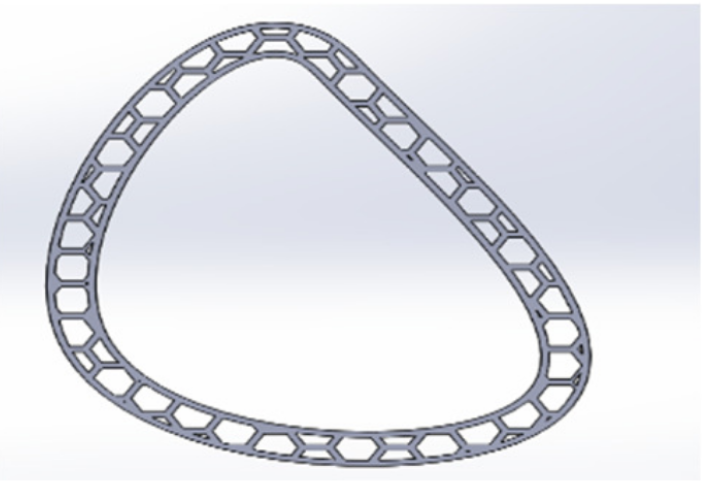
\includegraphics[scale=0.4]{Images/pomelo.png}
    }
    \qquad
    \subfloat[Hedgehog quill section.\label{fig:hedgehogstruct}]{
        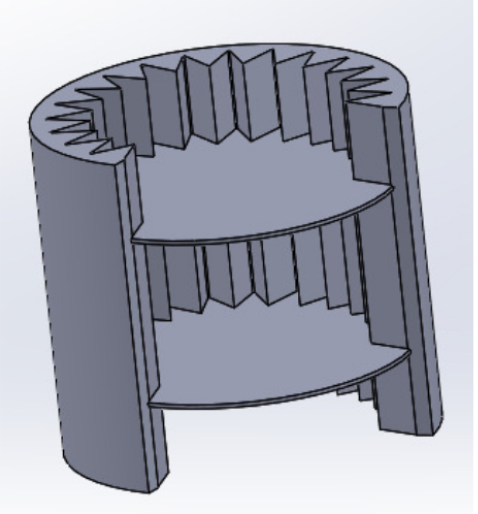
\includegraphics[scale=0.4]{Images/edgehog.png}
    }
    \qquad
    \subfloat[Section of a banana petiole.\label{fig:bananostruct}]{
        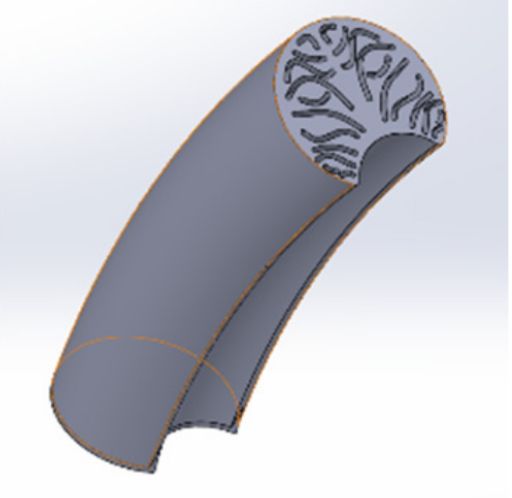
\includegraphics[scale=0.4]{Images/banano.png}
    }
    \caption[Cellular materials in nature]{Some examples of cellular materials in nature. Adapted from \citeauthor{mcnulty_framework_2017} (\citeyear{mcnulty_framework_2017}).}
    \label{fig:cellstruct}
\end{figure}
Lattice structures are versatile and can be effectively applied in various engineering fields to address multiple challenges. Specifically, they are commonly used in four main areas \cite{bhate_classification_2019}: structural engineering for vibration control, strain isolation, and weight reduction purposes; thermal engineering for applications such as heat exchangers, flame arresters, or heat shields; fluid dynamics engineering, where lattice structures can serve as catalyst carriers or packaging; and in biological engineering, where they can be leveraged for bone integration in prosthetic and cell growth. Due to their unique properties, lattice structures are an attractive choice for engineers and designers seeking innovative solutions to complex problems across a wide range of industries, especially in the automotive, aerospace, energy and commodities, and medical industries.
\subsection{Successful Case Studies for Lattice Structures} \label{subsec:casestudieslattice}
In this section, we will discuss some relevant case studies of successful applications of lattice structures. We will not focus on a single industry but rather analyze applications in various fields.
\section{Defects in 3d-printed metal objects}
\subsection{Classical indicators for lattice structures quality}